\section{Method} \label{sec:method} 


\subsection{Baseline Methods}

In order to gauge the efficiency of our deep learning approaches, we have
chosen to implement some baseline methods. These methods were picked
based on their performance in a previous project written by us as well,
\cite{US}. Albeit that project was only concerned with English texts
provided by the \cite{pan:2015}, and \cite{pan:2014} text forensics tasks,
we hypothesize that the performance of these approaches will perform just
as well on Danish texts.


\subsubsection{Extended Delta Method}

One of the best performing methods of \cite{US} was the extended delta method.
As the name suggests the method extends the already existing delta method
described by \cite{evert2015towards}. The normal delta methods consists of first
extracting word frequencies from all texts and using these as the describing
features. After doing this to the entire sample-space of texts, and applying a
linear transformation to their respective feature-sets, \gls{KNN} is then used
to determine the author of the introduced texts based on its closest neighbors
in the word-frequency feature-space. The extended delta method, simply expands
on the set of possible features to pick from, rather than being limited to only
using the word-frequencies of the text.


\subsubsection{Author Specific SVM}

Another algorithm used in \cite{US}. Heavily inspired by \cite{hansen2014}
starts out by fetching all texts known to be written by a specific author and an
equal number of texts known not to be written by that same author. It is upon
the feature-set extracted from these texts that a \gls{SVM} is trained, allowing
it to learn the specifics authors writing style from the known texts supplied
and in contrast what the writing style of someone not him is. When a new text,
with disputed authorship is presented the hope is that the trained \gls{SVM}
will be able to determine if the author it was trained on, is in fact the author
of this new text as well.


\subsection{Siamese Neural Network}

A Siamese Neural Network is a network architecture that shares weights across
multiple parts of the network. They have previously been used successfully for
comparison of objects in images by \cite{Koch2015SiameseNN}. They were
originally introduced by \cite{NIPS1993_769} who used them for verification of
signatures. \cite{NIPS1993_769} used the network to verify the authorship of
signatures which is very similar to what we are doing in this thesis. The
networks were supposed to learn how to extract features from the signatures and
a distance function was used on top of the networks to compare the computed
features. As descried earlier \cite{qian:2018} used a Siamese network for
authorship attribution but his network is also closely related to the authorship
verification case.

Our idea for our first network architecture was to use a similar architecture as
the ones above to extract features from a text. We start by preprocessing our
input data. The input consists of a set of utf-8 encoded texts with an
associated author id. To limit the number of different characters our network
has to deal with we map all characters that occur with a frequency of less than
$\frac{1}{100,000}$ to a garbage character we define. Since our network can only
handle inputs of the same length we pad all texts to have the length of the
longest text with another garbage character. We map all other characters to the
numbers 1 to the size of the character set.

Now we have a set of vectors of numbers of the same size each associated with an
author id. To construct an authorship verification dataset we looped through all
the vectors for each vector we drew a random vector of the same author and a
random vector of a different author. We then created two problem instances we
could train on. One instance of two vectors from the same author with a label of
1 and one instance of two vectors from different authors with a label of 0. We
split the list of problems into two sets. A validation set consisting of 20\% of
the problems and a training set consisting of 80\% of the problems.

The network we used to try and solve the problem is shown in Figure
\ref{fig:network_one}. The Siamese part of the network is the Convolutional
Layer. We used 1000 filters of size 10. That means that 1000 different features
are supposed to be learned by the network and each feature can use a local
context of 10 characters to extract a feature. After the convolution we have a
max-over-time pooling layer. The layer takes the maximum value of each feature
such that we have 1000 features from each text. We then have a normal dense
neural network on top of that which are given the features of both texts. The
dense network is then supposed to learn how to compare the features from the
two texts. We have 2 dense hidden layers each with 500 neurons. At the end we
have a output layer with two outputs. The activation function for all layers
except the last one is the rectified linear unit and the activation function of
the last layer is the softmax function. The output of the network is a
probability distribution over the two classes.

The input to the network first goes through an embedding layer. The embedding
layer transforms integers into dense vectors of floating point numbers. The
embedding layer functions as a lookup table such that each integer is mapped
to the same dense vector. The embedding is trainable meaning that better
embeddings will be learned while the network is training.

\begin{figure}[htb]
\centering
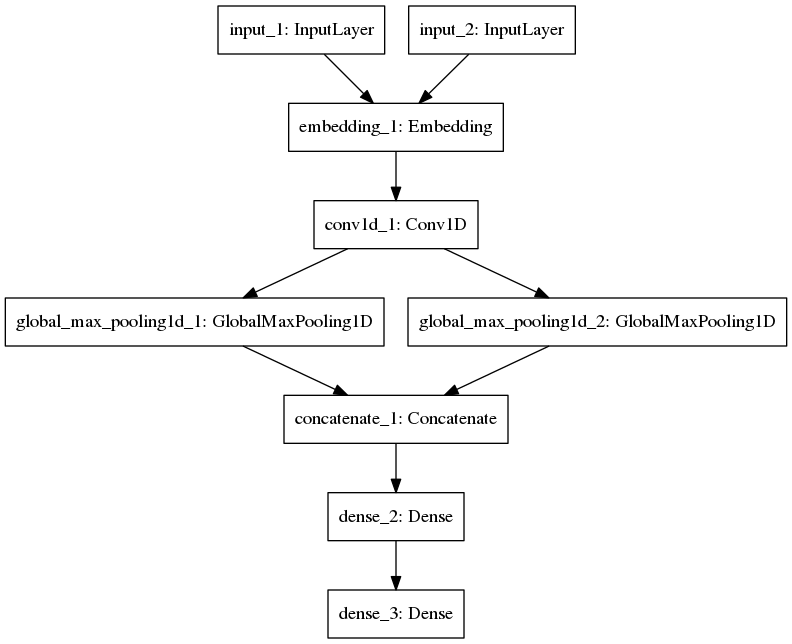
\includegraphics[scale=.4]{./graphs/method/siamese.png}
\caption{Don't worry, this will be prettier later. Shows the structure of our
    first Siamese Neural Network implementation.}
\label{fig:network_one}
\end{figure}

The results of the network with the best validation accuracy is,

Validation accuracy 0.6868421052631579

Validation true positives 269

Validation true negatives 253

Validation false positives 109

Validation false negatives 129

TODO:
\begin{itemize}
    \item We would like to experiment more with different functions to combine
        the features outputted from the convolutional layers. Currently we
        concattenate them maybe we could combine them with an absolute
        difference or something else.
    \item We would like to experiment with convolutional filters that does not
        look at 10 characters at a time. And maybe include both "longer" and
        "shorter" filters which can learn from different levels.
    \item We would like to not use a dense layer on the top of the feature
        generation but a simple distance metric as some of the other articles
        did.
    \item Add dropout to combat overfitting.
    \item Use more data in the training to combat overfitting.
\end{itemize}
